
\section{Session 2. Nonlinear Optimization}


Example Production cost:

    A company aims at minimizing the production cost during a series of production periods of time $T_i$, characterised by the demand $D_ii$, equipment capacities and material limitations $E_i$, labor force $L_i$ (which cost depends quadratically on the difference of labor force between two periods $C_L(L_i-L_{i-1})^2$), productivity of each worker $P_i$, the number of units of inventory at the end of each production period $I_i$ and the cost to bring them to the next production period $C_I$.

  \begin{center}
    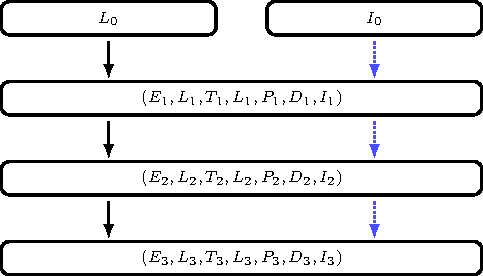
\includegraphics[width=0.4\textwidth]{ProductionSchedule.pdf}
  \end{center}
%------------------------------------------------%------------------------------------------------

  The problem, as stated, aims at minimizing the function:
  \[f(\vec{L},\vec{I})=\sum_{i=1}^T C_L (L_i-L_{i-1})^2+C_I I_i\]
  subject to:
  \[
  \begin{cases}
    L_iP_i \leq E_i\\
    I_{i-1}+L_i P_i \geq D_i\\
    I_i = I_{i-1} + L_i P_i -D_i\\
    L_i,I_i \geq 0, \; \forall i=1,\ldots,T
  \end{cases}
  \]
  Quadratic objective function with linear constraints.

%------------------------------------------------%------------------------------------------------

\begin{itemize}
  \item We want to obtain the best solution to a mathematical programming problem in which both  objective function and constraints have general non-linear forms.

  \item Most of the problems are non-linear indeed!

  \begin{itemize}
    \item Unconstrained Problems (often dealt with differential calculus)
    \item Constrained Problems (may include systems of equations to be solved)
  \end{itemize}

  \item Classical underlying mathematical theories do not necessarily provide practical methods suitable for efficient numerical computation.

  \item Points of optimality can be anywhere inside the problem boundaries

  \item No methods applicable to all non-linear problems
\end{itemize}
%------------------------------------------------%------------------------------------------------

\subsection{Some theoretical background}

material: convex and non linear problem.pdf

\subsection{Feasible region}

   Set of points satisfying all the constraints (the area between constraint boundaries).


 \begin{center}
  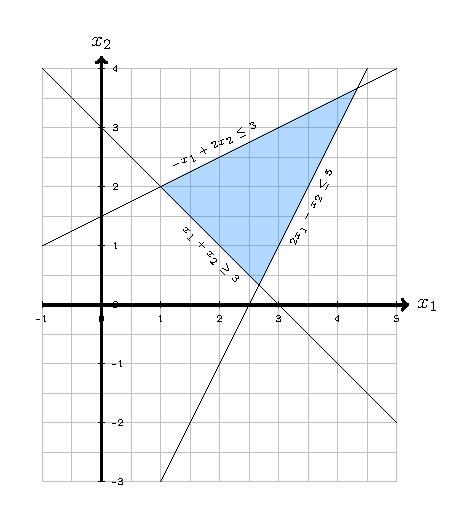
\includegraphics[width=0.6\linewidth]{feasibleregion.pdf}
 \end{center}


  \begin{center}
    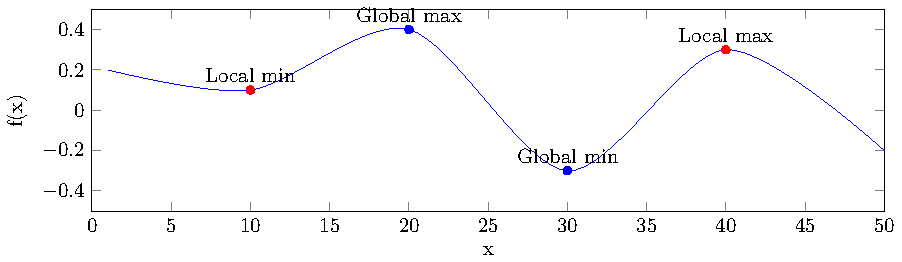
\includegraphics[width=0.6\textwidth]{globalminmax.pdf}
  \end{center}

  A local maximum of the function $f(x)$ exists in $x^*$ if there is a small positive number $\epsilon$ such that
  \[
    f(x^*)>f(x), \; \forall x\in\mathbf{R} : \|x-x^*\| < \epsilon
  \]
  A global maximum of $f(x)$ exists in $x^*$ if
  \[
    f(x^*) > f(x), \; \forall x\in\mathbf{R}
  \]
  (analogous definitions for local/global minimum)
%------------------------------------------------%------------------------------------------------

\subsection{Concavity/convexity}

  For a continuous convex function, given any two points $x_1$ and $x_2$:
  \begin{equation}
  f[\lambda x_1 +(1-\lambda)x_2] \leq \lambda f(x_1) +(1-\lambda) f(x_2), \; 0 \leq \lambda \leq 1
\label{eq:convex}
\end{equation}
    (analogous situation for a continuous concave function)
  \begin{center}
    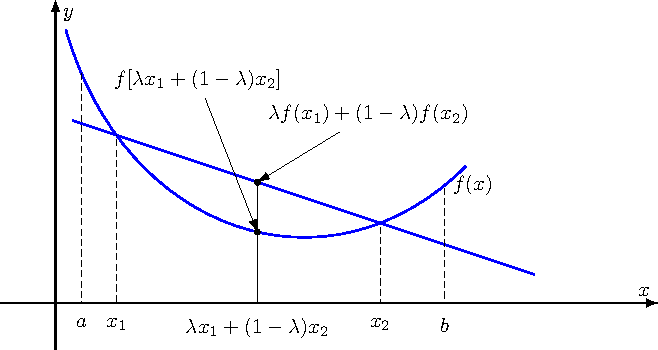
\includegraphics[width=0.6\textwidth]{concave.pdf}
  \end{center}


    The term "convex" can be applied both to sets and functions. A set $S\in \mathbf{R}^n$ is a {\it convex set} if the straight line segment connecting any two points in $S$ lies entirely inside $S$.

Note that $f(x)$ is a convex function if its domain $S$ is a convex set and if for any two points $x_1$ and $x_2$ in $S$ Eq. \ref{eq:convex} holds.

\begin{Exercise}
  Can you draw a convex function that depends on two variables, $f(x,y)$? Can you generalize Eq. \ref{eq:convex}?
\end{Exercise}


%------------------------------------------------%------------------------------------------------
  \begin{itemize}
    \item If a convex nonlinear function is to be optimized without constraints, a global minimum may occur when $f'(x)=0$. Not always this is the case:
    \begin{center}
      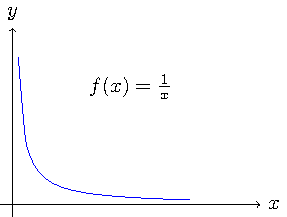
\includegraphics[width=0.5\textwidth]{1overx.pdf}
    \end{center}
    \item If the feasible region for a nonlinear programming problem is convex, each of the constraint functions is convex and are of the form $g_i(x)\leq b_i$
  \end{itemize}
%------------------------------------------------%------------------------------------------------
\begin{itemize}
    \item A local minimum is guaranteed to be a global minimum for a convex objective function in a convex feasible region, and
    \item a local maximum is guaranteed to be a global maximum for a concave objective function in a convex feasible region.
  \end{itemize}
  Many functions in nonlinear programming problems are neither concave nor convex!
  \begin{Exercise}
    Is the function $f(x)=x^2$ convex? Are the regions defined by $x^2=4$ or $x^2\geq 9$ convex?
  \end{Exercise}

    \begin{Exercise}
    Are the functions $f(x,y)=3x^2-2xy+y^2+3e^{-x}$ and $g(x,y)=x^4-8x^3+24x^2-32x+16$ convex? 
  \end{Exercise}
%------------------------------------------------%------------------------------------------------

  \begin{Exercise}
    Consider these two nonlinear problems\cite{carter_operations_2019}:
    \begin{center}
      \begin{tabular}{cc|cc}
        minimize & $f(x,y)=x-2xy+2y$ & minimize & $f(x,y)=x-2xy+2y$\\
        subject to & $\begin{cases}x^2+3y^2\leq10\\3x+2y\geq 1\\x,y\geq 0\end{cases}$ & 
        subject to & $\begin{cases}x^3-12x-y\geq 0\\x\geq 1\end{cases}$
      \end{tabular}
    \end{center}
    Are their feasible regions convex?
   \end{Exercise}
%------------------------------------------------%------------------------------------------------

  \begin{align}
  (\Hessian f)_{ij} &\equiv \frac{\partial^{2} f}{\partial x_{i} \partial x_{j} } \\
  \Hessian\left( \frac{x^{2}}{y} \right) &=
  \begin{bmatrix}
    \frac{2}{y} & - \frac{2x}{y^{2}} \\
    -\frac{2x}{y^{2}} & \frac{2x^{2}}{y^{3}}
  \end{bmatrix}
\end{align}

